\section*{Reviewer 1}

\paragraph{R1.1} We have extended the introduction to discuss the advantages and disadvantages of PSG and why it is not applicable to our
problem. Thanks for the comments.

\paragraph{R1.2} Embarrassed not to have introduced and provided sufficient details on our pilot study. This information is now given in Section 3.

\paragraph{R1.3} We take 12-28 samples every minute to detect respiratory events. This is based on the observation that an adult typically
breathes around 15 times per minute. We found that this setting is effective for our problem. This is now clarified in Section 2.1.

\paragraph{R1.4} The 10 volunteers involved in the training data process (pilot study) for determining the algorithm parameters are different from the 15 users recruited in our
evaluation. The data were collected while they were sleeping. This is clarified in Section 2.1 in the revised manuscript.

\paragraph{R1.5} Our HMM model is trained using the training data. This is now clarified in Section 2.4. See also R1.4.
\vspace{-2mm}
\paragraph{R1.6} To evaluate our approach, we have randomly picked at least 3 sets of data from each of our 15 testing users.
The current submission is not evaluated on the full dataset (videos of a over 1,000 hours) due to the time constraint (as we need to watch
each video to mark sleep events). That said, we are able to demonstrate the usefulness of our approach on a relatively small but
representative set of data. We are currently working to extend our evaluation to the entire dataset. The results will be ready for and
included in the camera ready paper.

\paragraph{R1.7} ``invasive" is indeed a poorly chosen word for describing Fibit. We have reworded.
\vspace{-2mm}
\paragraph{R1.8} The signals shown in Fig.5 are from a single subject. This is clarified in the revised version.

\paragraph{R1.9} \textcolor{blue}{Our work detect the position of hand, and the use of respiratory events can help us to distinguish chest/abdomen from shoulder/hip. Fig. \ref{Bodyhand} showed the angle change value measured by the gyroscope, when the hand moves from the side of the body to the chest and the shoulders. We found that their trajectories are very similar, which makes it difficult to distinguish between these two positions, but the obvious respiratory events cannot be observed when the hand is put on the shoulder.}

\begin{figure}[!t]
	\centering
	\subfigure[]{\label{BodytoChest}
		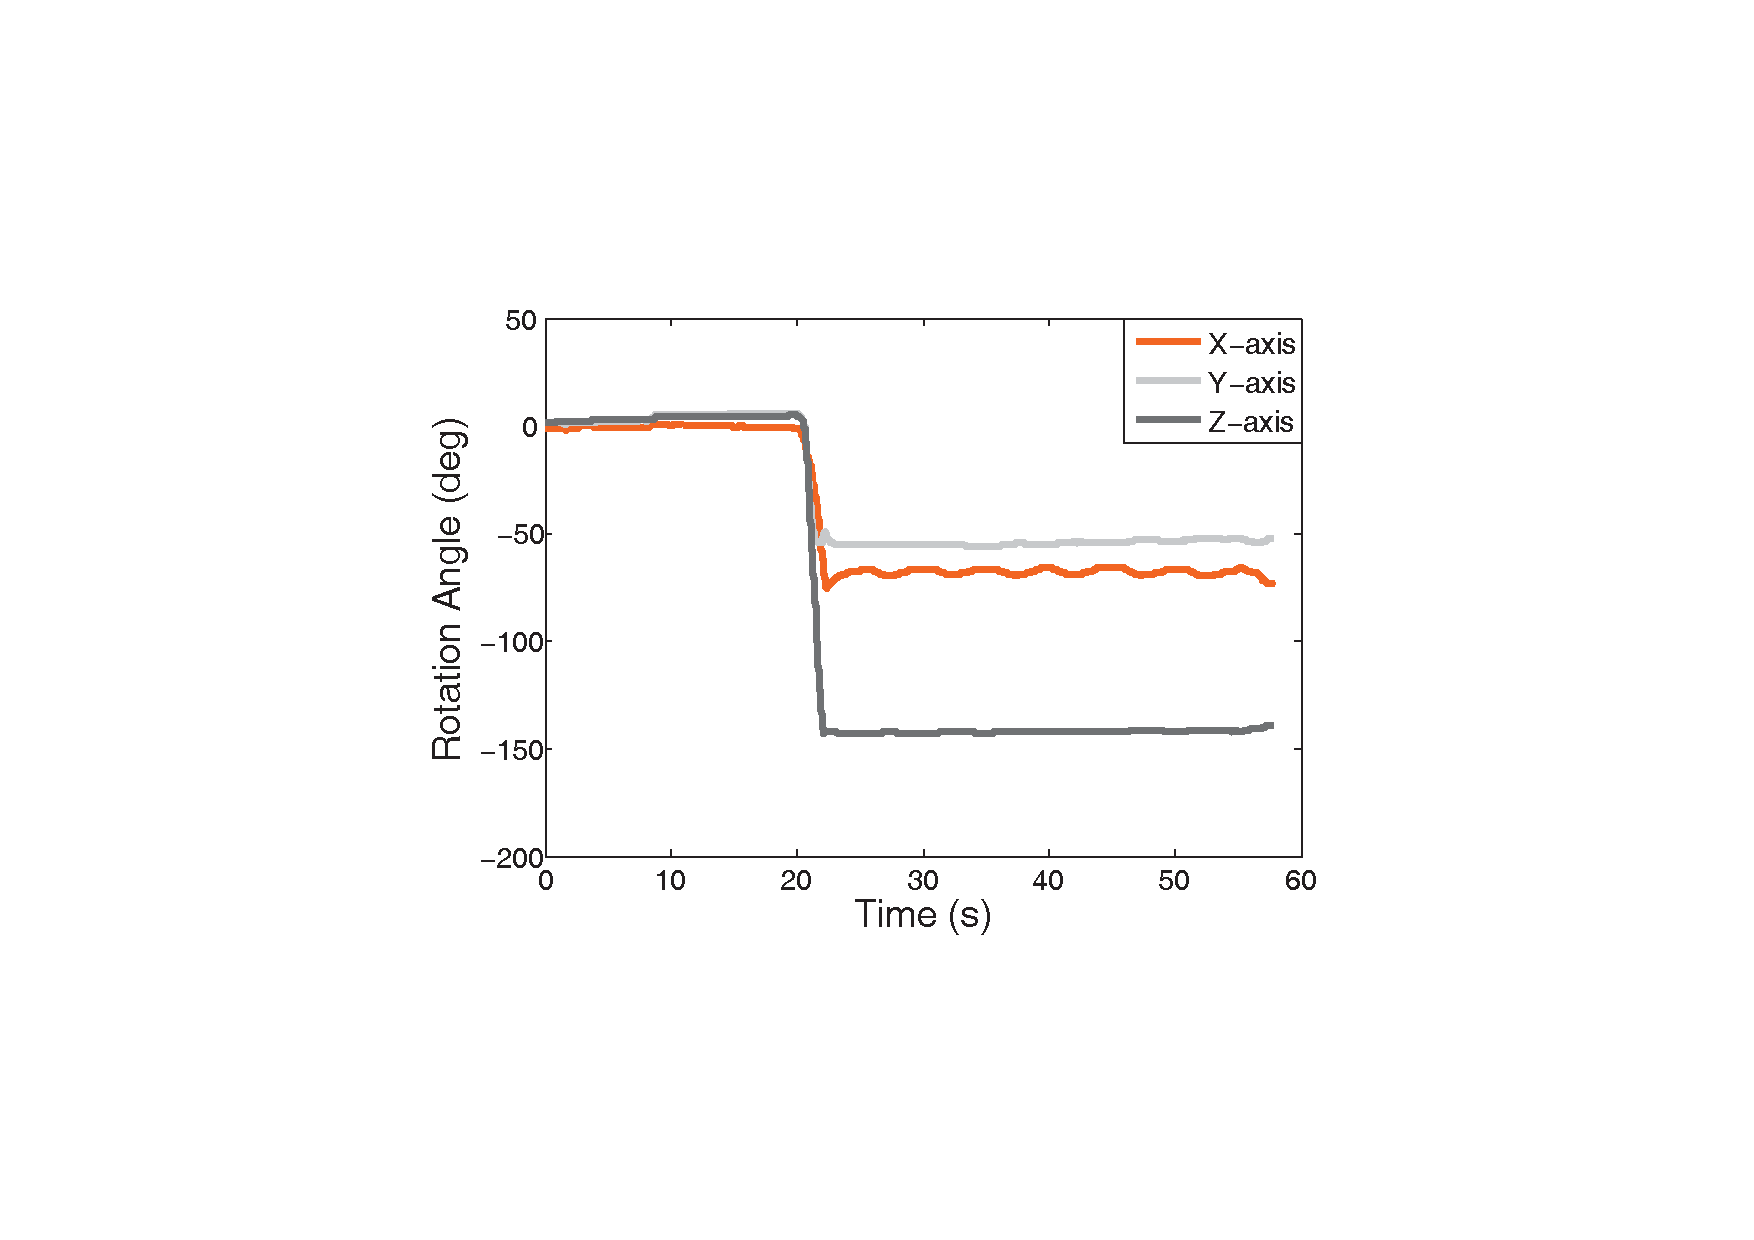
\includegraphics[width=0.32\linewidth]{Figures/BodytoChest.pdf}}
	%  \hfill
	\subfigure[]{\label{BodytoShoulder}
		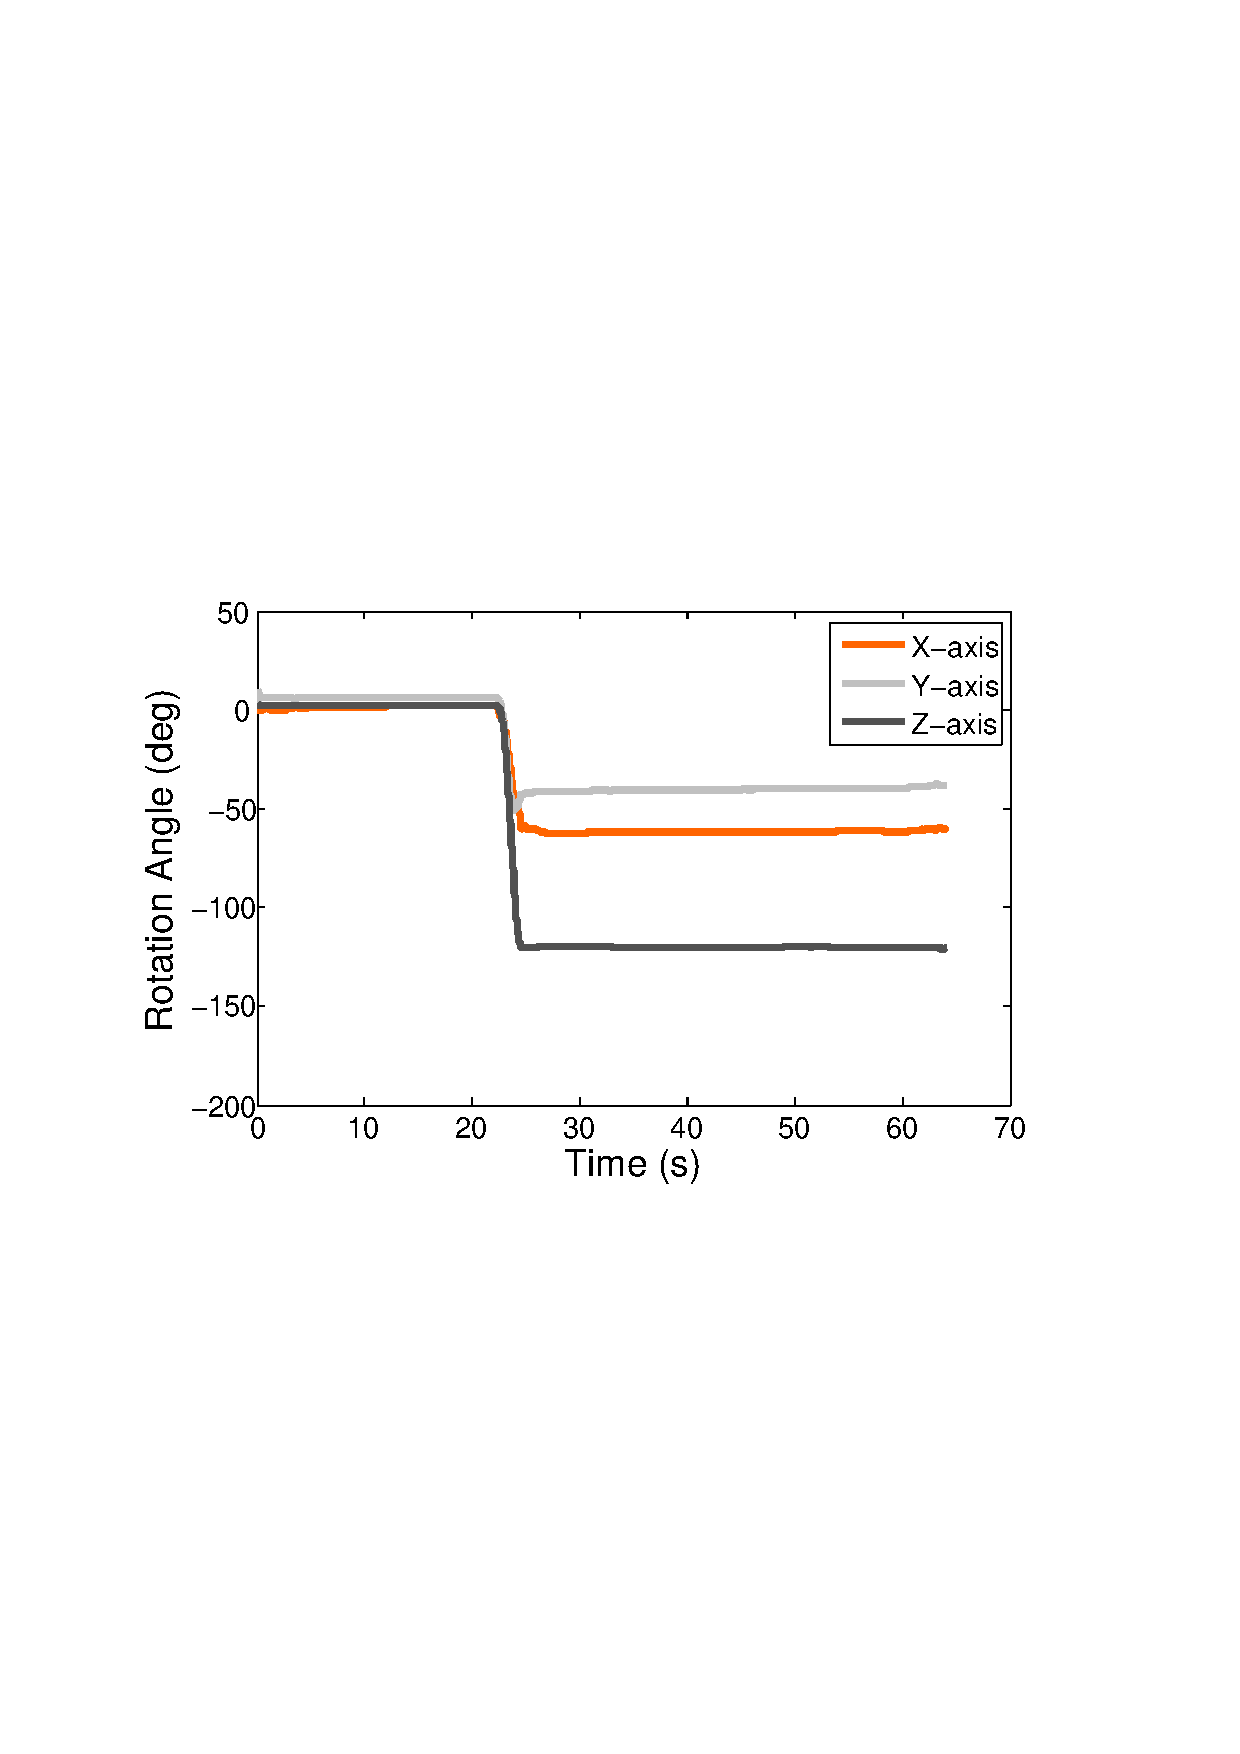
\includegraphics[width=0.34\linewidth]{Figures/BodytoShoulder.pdf}}
	\caption{The characteristics of hand movement from the position beside the body  to (a)  the chest, and (b) the shoulder.}\label{Bodyhand}
\end{figure}


\paragraph{R1.10} Good catch, the sentence should be instead read as ``A body rollover event is recorded when the posture changes are detected between
two time points". We have now corrected the phrase.

\paragraph{R1.11} We have given the parameters for the moving average filter and explain how they are obtained in Section 2.1 in the revised version.

\paragraph{R1.12} The acceleration threshold was determined from our training data. This is now clarified in Section 2.1. See also
R1.4.

\vspace{-2mm}
\paragraph{R1.13} Our algorithm does consider a situation where the wrist turns so that the back of the hand become downward. This is now clarified in Section 2.3.

\paragraph{R1.14} Yes, there is no standard definition for sleep stages. We have provided our definitions of the various stages (per reviewer suggestions) in Section 2.4.

\paragraph{R1.15} We have extended Section 5 to discuss how our approach can be extended to a multi-sleeper scenario.

\paragraph{R1.16} The ground truth of micro-body movements are obtained through (a) watching videos and (b) using the phone accelerometer data. We use the accelerometer data is because visions of subtle body movements may be blocked due to camera angles or surrounding objects e.g., quilt. This is clarified in Section 4.1.4.

\paragraph{R1.17} We have provided a more detailed analysis and discussion for Table 9 in Section 4.2.4.

\paragraph{R1.18} Having a discussion on the frequency of unusual arm positions is a great point. This is now included in Section 5.

\paragraph{R1.19} We have make all the minor corrections and fixed the presentation issues. Many thanks for the feedback.
